% !TEX root = ../SYSprojektrapport.tex
% SKAL STÅ I TOPPEN AF ALLE FILER FOR AT MASTER-filen KOMPILERES 


\label{Modelopbygning}
I dette kapitel beskrives modellen og det underbyggende data, der anvendes til simuleringen af de omtalte cases. Modellen valideres igennem spændingsfalds- og kortslutningsberegninger.

\section{Model}

For at undersøge husstandsbatterier indflydelse i et elnet er der simuleret 5 byer med ca. 2000 hustande, der alle har et batteri installeret. Hver husstand er sat til at have et gennemsnitligt dagligt forbrug på 14kWh\footnote{https://orsted.dk/Privat/Faa-en-lavere-regning/Kom-godt-i-gang-og-spar-paa-energien/Test-dit-gennemsnitsforbrug/Elforbrug}. Det giver et gennemsnitlig forbrug på 1183kW per by. For at finde en realistisk maksimal belastning er der taget udgangspunkt i Energinets belastnings- og produktionsinformation for Danmark\footnote{https://www.energidataservice.dk/da\_DK/}. Det er undersøgt hvor stor en del den gennemsnitlige belastning i modellen udgør af Danmarks gennemsnitlige belastning og derved fundet en skaleringsfaktor på 716. Denne skaleringsfaktor er brugt til at finde den samlede maksimale belastning for byerne ved dividere Danmarks maksimale belastning med faktoren. Den maksimale belastning for hver by ligger derved på 1524kW. \\
På figur \ref{fig:Simdis} ses distributionsnettets opbygning der er lavet som en ringforbindelse fra \textit{Distribution busbar}, med en ekstra tværgående linje. Ved hver by er placeret en transformer der transformere spændingen fra 10kV til 0,4kV. Hver by er simplificeret til en belastning, et batteri og et solcelle anlæg. Den maksimale batteri kapacitet er fundet i forhold til at hver hustand har monteret en Tesla powerwall, der kan levere 5kW, så hver by har en batteri kapacitet på 10000kW. Den maksimale solcelle produktionsmængde er fundet ud fra Energinets oplysninger for hele landet og derefter divideret med skaleringsfaktoren, som giver en maksimal produktion på 912kW per by. 

 
 \begin{figure}[H] % (alternativt [H])
 	\centering
 	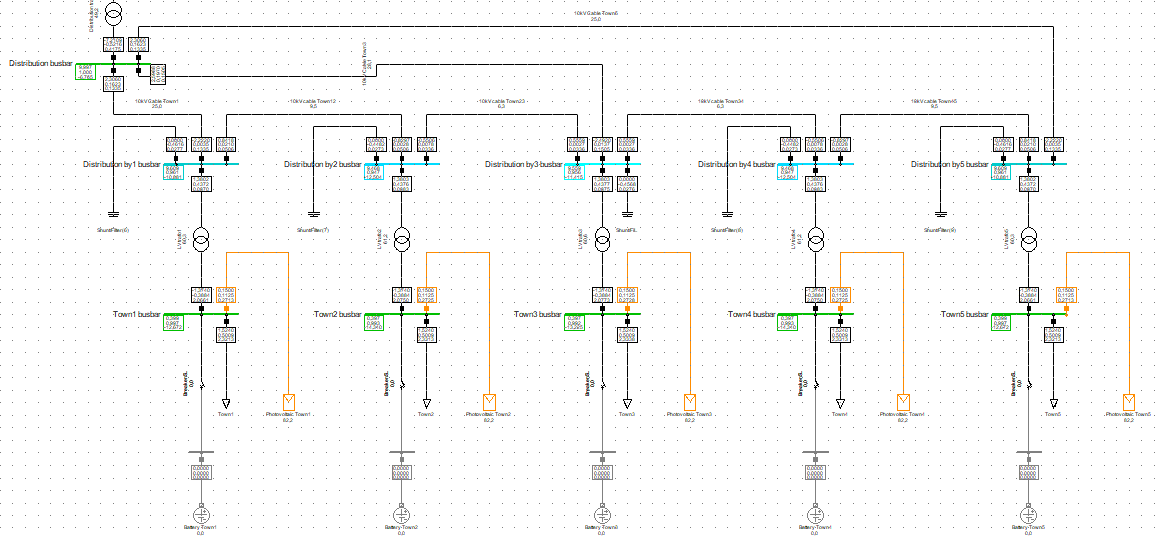
\includegraphics[width=1\textwidth]{figurer/Sim_model_2}
 	\caption{Systemets belastning og distribution}
 	\label{fig:Simdis}
 \end{figure}
    

På figur \ref{fig:SimTrans} ses transmissionsnettet. For at simplificere modellen er al vind- og fossil energi samlet i to generatorer. Størrelsen af vind generatoren er valgt ud fra den gennemsnitlige produktion af vindenergi i Danmark. Vindmølle generatoren producerer derved 2MW. Den fossile generator er sat som referencemaskine og ændre sin produktion i forhold til belastningen i nettet. Energien transformeres først op til et 150kV transmissions net og derefter til 60kV. 60kV transmissionen er lavet med 2 redundante kabler så det kan undersøges hvad der sker, hvis det ene kable falder ud. Til sidst transformeres spændingen ned til distributions niveauet. Ydermere er der placeret en stor batterienhed på 60kV busbaren for at kunne undersøge forskellen mellem husstandsbatterier og en centralt placeret batteripark.

Generatorer, kabler og transformere er lavet som simplificeret modeler med generelle værdier for de enkelte komponenter samt tilpasset for spænding og belastning i de forskellige niveauer.
 

\begin{figure}[H] % (alternativt [H])
	\centering
	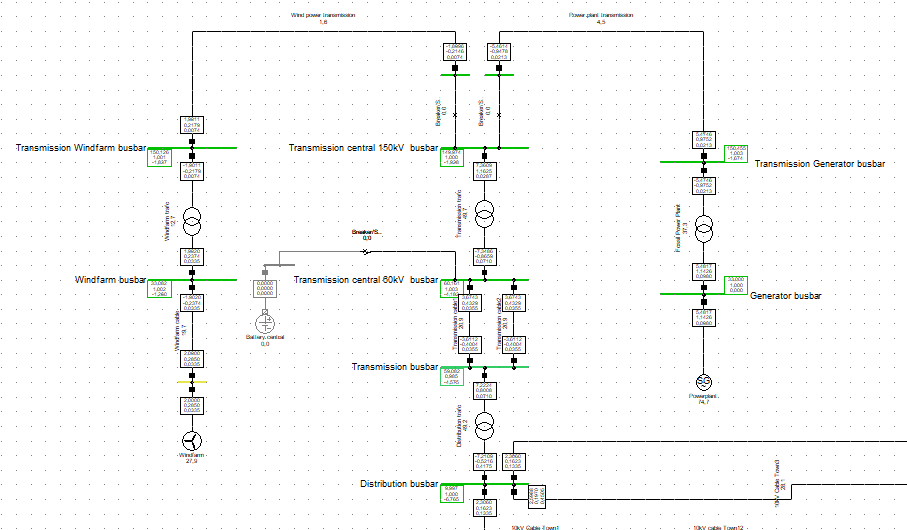
\includegraphics[width=1\textwidth]{figurer/Sim_model_1}
	\caption{systemets produktion transmission}
	\label{fig:SimTrans}
\end{figure}
